\documentclass{beamer}
\usetheme{Warsaw}
\useinnertheme{circles}
\useoutertheme[subsection=false]{smoothbars}
\usepackage[utf8x]{inputenc}
\usepackage[czech]{babel}
\usepackage[T1]{fontenc}
\usepackage{listings}
\usepackage{tikz}
\lstset{basicstyle=\tiny\ttfamily}
\logo{
\includegraphics[height=0.5cm]{brmlab.pdf}}

\begin{document}

\AtBeginSection[]
{
  \begin{frame}
    \frametitle{Outline}
    \tableofcontents[currentsection]
  \end{frame}
}

\title{brmiversity: Umělá inteligence\\a teoretická informatika}
\subtitle{Přednáška č. 2}
\author{Petr Baudiš $\langle${\tt pasky@ucw.cz}$\rangle$}
\institute{
	brmlab 2011\\
	\vskip 1ex
	\pgfdeclareimage[height=4ex]{ccbysa}{by-sa.pdf}
	\pgfuseimage{ccbysa}
}
\date{}
\frame{\titlepage}

\section{Úvod do neurofyziologie}

\subsection{}
\begin{frame}{Neuron}
\begin{columns}
\begin{column}{6cm}
\begin{itemize}
\item Divná buňka: Axon, dendrity a~tělo neuronu
\item Na axon jsou napojené dendrity cizích neuronů --- synapse (excitační, inhibiční)
\item Biologické neuronové sítě bývají {\em husté} (86 miliard neuronů, 1~trilion synapsí)
\item Elektrický signál se přenáší iontově; charakteristický průběh a frekvence
\end{itemize}
\end{column}
\begin{column}{5cm}
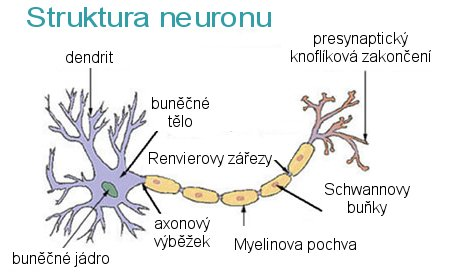
\includegraphics[width=5cm]{Neuron-cs.jpg} \\
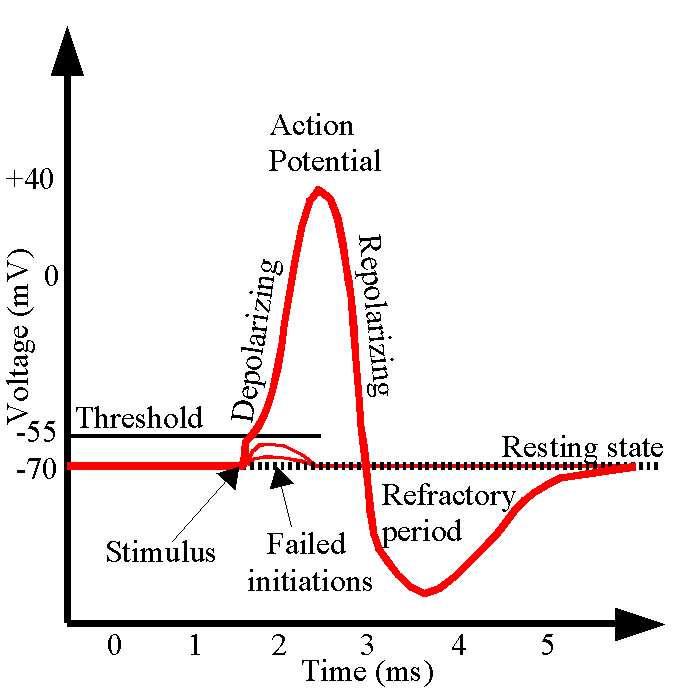
\includegraphics[width=5cm]{ActionPotential.png}
\end{column}
\end{columns}
\end{frame}

\subsection{}
\begin{frame}{Neuronové obvody}
\begin{columns}
\begin{column}{5cm}
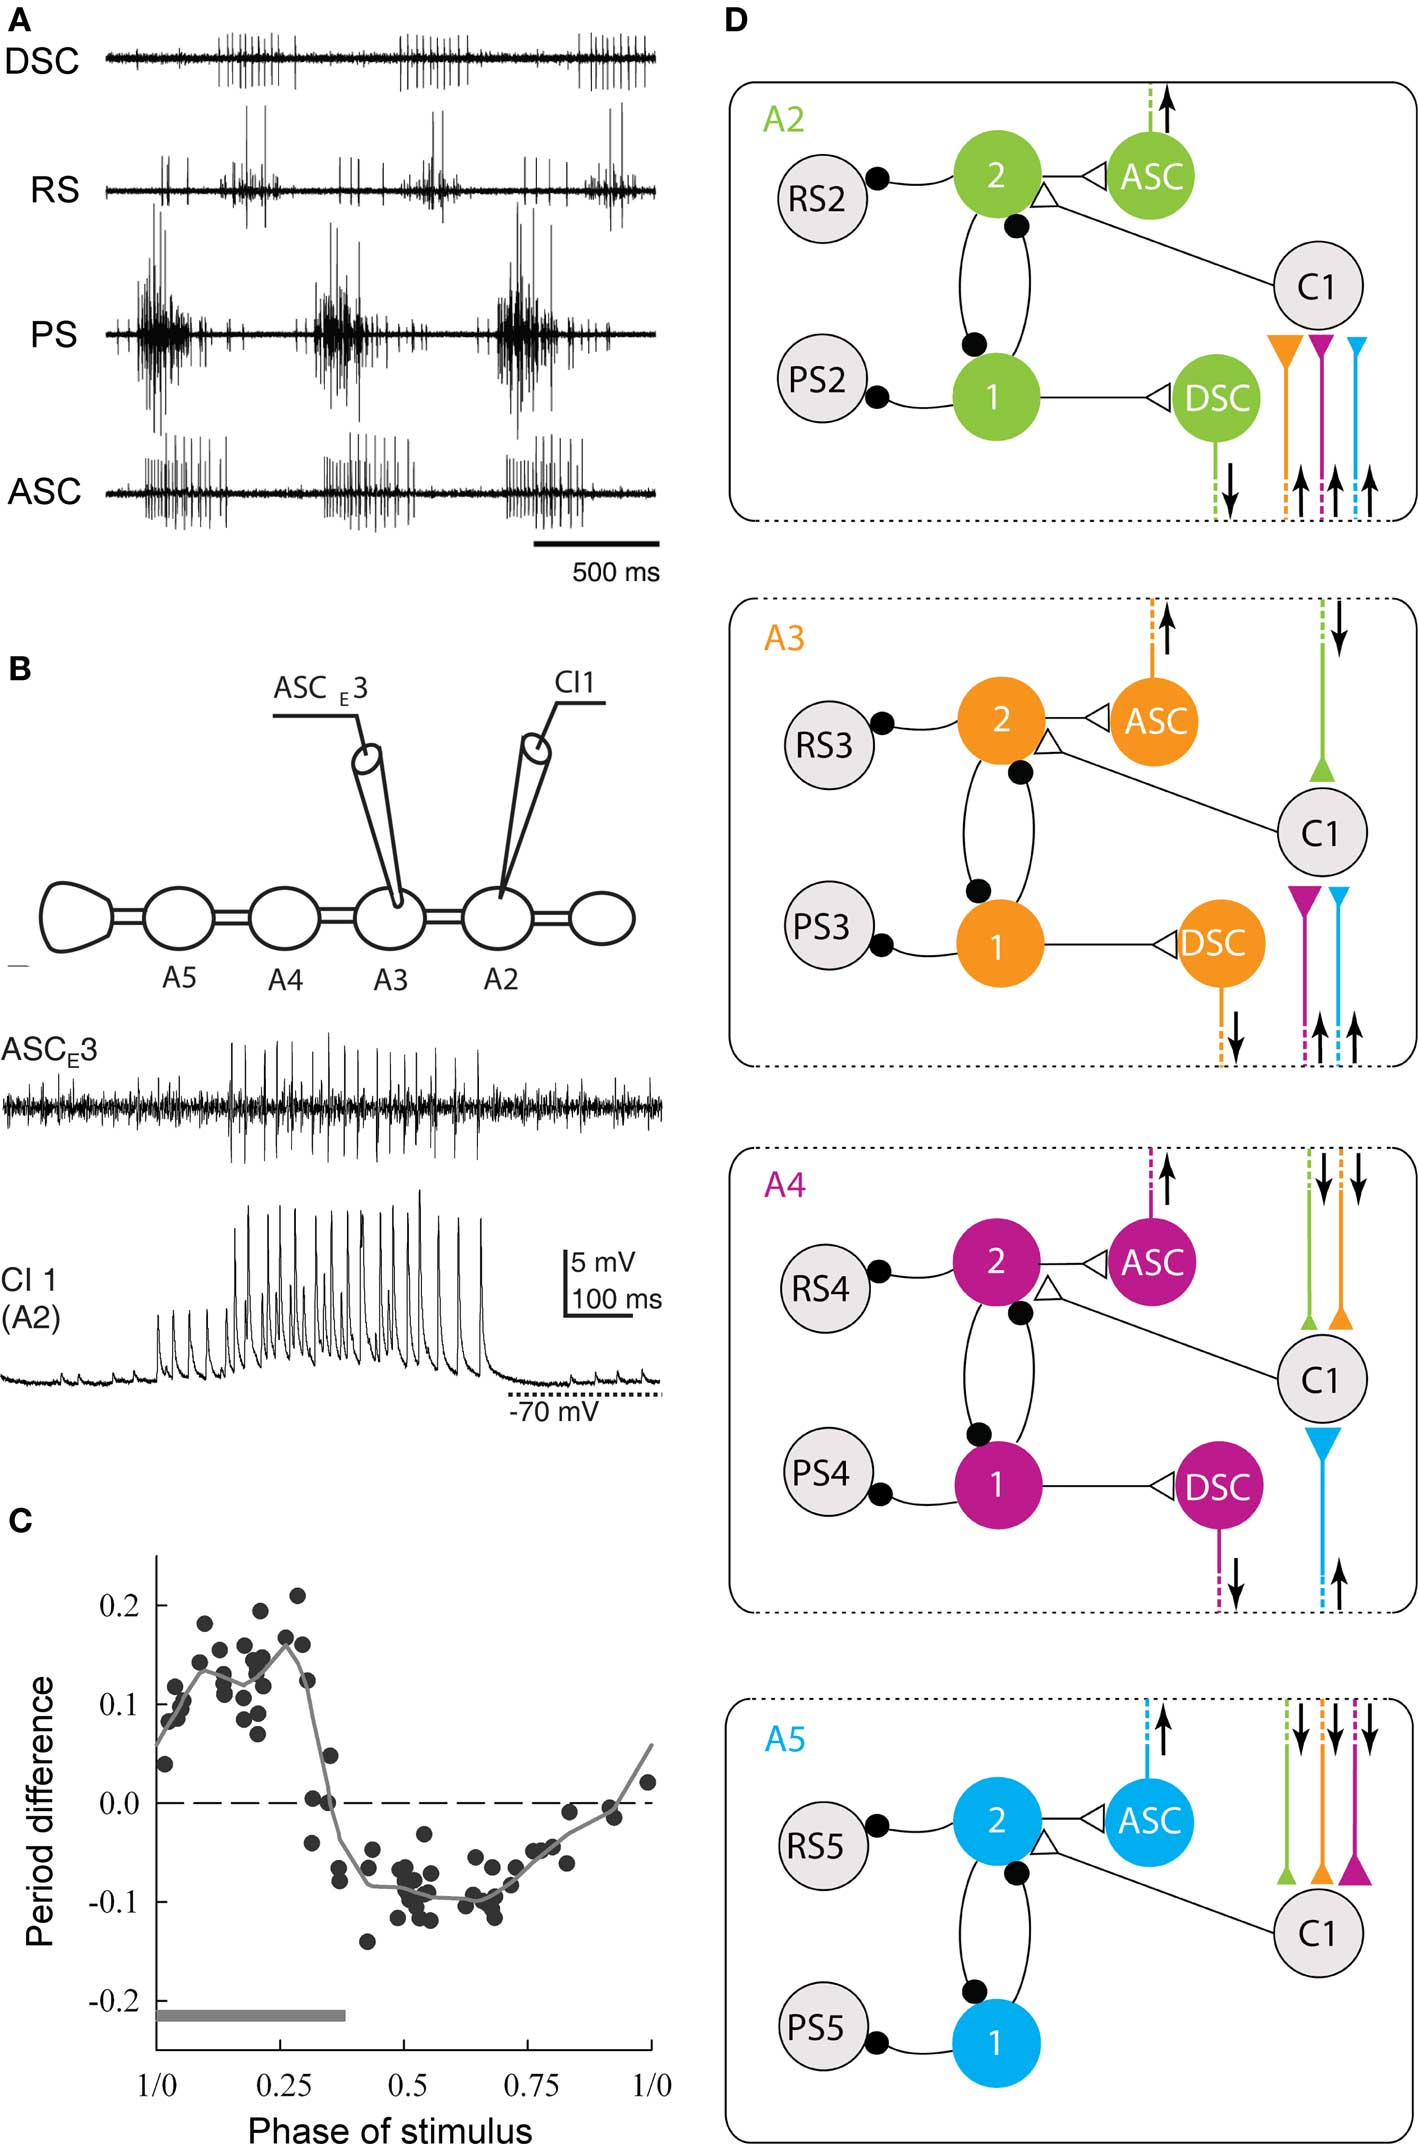
\includegraphics[width=5cm]{fnbeh-04-00045-g003.jpg}
\end{column}
\begin{column}{6cm}
\begin{itemize}
\item Zejména v míše a jinde v těle ``lokální processing''
\item Signálu může trvat cesta z periferie do mozku a zpět stovky milisekund
\item Reflexy, generátory plánovaného pohybu a builtin pattern generátory přímo v míše
\item Relativně dobře prozkoumáno několik instancí; vlnění, chůze
\end{itemize}
\end{column}
\end{columns}
\end{frame}

\subsection{}
\begin{frame}{Mozek}
\begin{itemize}
\item Povrch --- šedá kůra (neurony), \\ vnitřek --- synapse
\item Technická infrastruktura --- gliové buňky
\item Zřejmě alespoň částečně specializovaný
\item Vizuální, aurální, motorický kortex
\item Další struktury --- hippokampus, mozeček, corpus callosum, prodloužená mícha, \dots
\end{itemize}
\begin{tikzpicture}[remember picture,overlay]
  \node [xshift=-4.5cm,yshift=-5cm,above right] at (current page.north east)
    {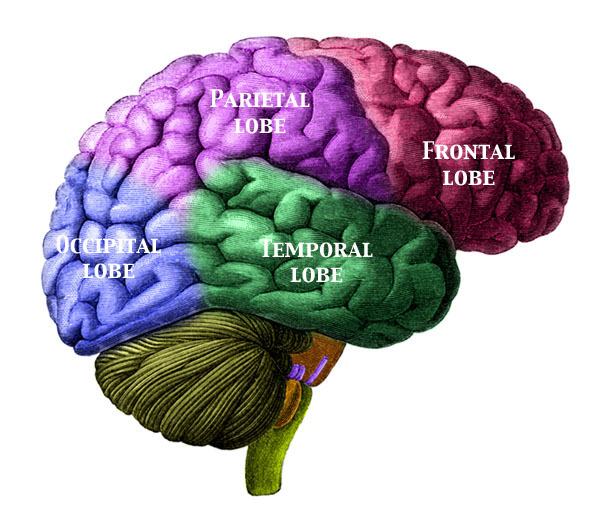
\includegraphics[width=4cm]{BrainLobesLabelled.jpg}};
\end{tikzpicture}
\end{frame}

\subsection{}
\begin{frame}{Zrak neurologicky}
\begin{itemize}
\item Sítnice --- tyčinky a čípky (bitmapa) a přímo pod nimi první laterální spoje
\item Do vizuálního kortexu již jdou preprocesovaná data (hranová mapa)
\item V1: Spatiálně odpovídá zornému poli, pattern matching, orientace, barva, hrany
\item V2: Funkčně podobná V1, částečně zaostřená dle pozornosti, souvislost s pamětí
\item V3: Zejména detekce pohybu.
\item V4: Ovládaná pozorností. Kromě featur V1 i geometrické tvary, spatiální souvislosti
\item Rozdělení není moc jasné, spoustu zpětných spojení, atd.
\end{itemize}
\end{frame}

\subsection{}
\begin{frame}{Hippokampus}
\begin{itemize}
\item Útvar uvnitř mozku ve tvaru \\ mořského koníka
\item Intenzivní výzkum --- orientace \\ v prostoru a paměť
\item Orientace v prostoru: ``Hexová mapa'',\\ head direction cells + grid cells = place cells
\item Paměť: Koordinace ukládání do dlouhodobé paměti,\\ pacient H. M.
\end{itemize}
\begin{tikzpicture}[remember picture,overlay]
  \node [xshift=-4.5cm,yshift=-4.6cm,above right] at (current page.north east)
    {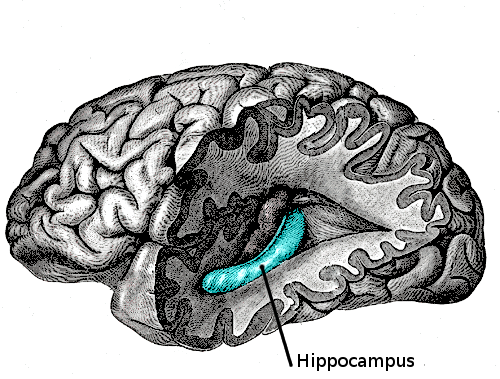
\includegraphics[width=4cm]{Gray739-emphasizing-hippocampus.png}};
\end{tikzpicture}
\end{frame}

\subsection{}
\begin{frame}{Umělé neuronové sítě}
\begin{itemize}
\item Neuron je lineární klasifikátor (``perceptron'')
\item Vstupy vynásobím váhami a sečtu, je výsledek vyšší než práh?
\item Více vrstev neuronů dokáže rozhodovat o složitějších charakteristikách vstupu
\end{itemize}
\end{frame}

\subsection{}
\begin{frame}{Otázky?}
\begin{center}
Příště: Umělý neuron a co dokáže
\end{center}
\end{frame}

\section{Základní algoritmy}

\subsection{}
\begin{frame}{Pointery a rekurze}
\begin{itemize}
\item Ukazatel --- proměnná obsahující pozici (``souřadnice'') v paměti \\
	Můžeme manipulovat jak s pozicí, tak s daty na oné pozici \\
	Můžeme mít i ukazatel na funkci (kód)!
\item Rekurze --- z funkce zavoláme sebe sama, typicky na určitou podúlohu \\
	$f(0) = 1 \qquad f(x) = x * f(x - 1)$
\end{itemize}
\end{frame}

\subsection{}
\begin{frame}{Hledání slova v textu}
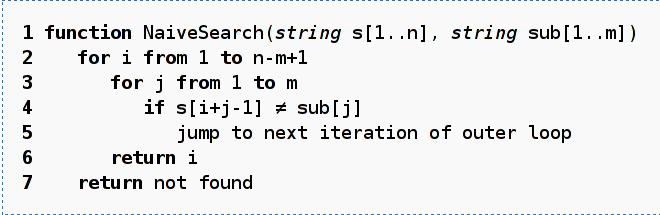
\includegraphics[width=10cm]{naive.png} \\
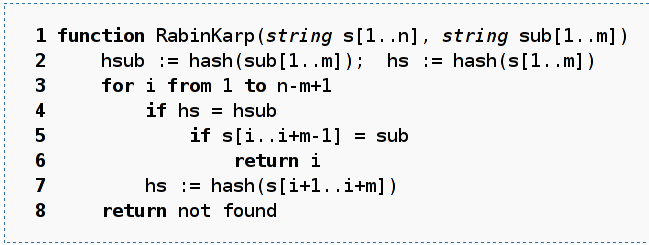
\includegraphics[width=10cm]{rabinkarp.png}
\end{frame}

\section{Vyčíslitelnost}
%     Turingův stroj, lambda kalkulus, rekurzivní funkce, brainfuck… «««<++++++

\subsection{}
\begin{frame}{Vyčíslitelnost}
\begin{center}
``Computer science is no more about computers than astronomy is about telescopes.'' \\
Edsger Dijkstra
\end{center}

Budeme zkoumat, co všechno dokážeme naprogramovat a ``sílu'' různých výpočetních modelů.
\end{frame}

\subsection{}
\begin{frame}{Algoritmicky vyčíslitelné funkce}
\begin{itemize}
\item Jak matematicky popsat program?
\pause
\item Série operací nad vstupem, které vyrábějí výstup (akceptor vs. transducer); data jsou čísla
\item Co je to operace a jak ji vyjádřit?
\pause
\item Operace --- aritmetika a ``control flow'' (podmínky, cykly, skoky)
\item Jsou transformace, které se nedají vyjádřit pomocí základní aritmetiky?
\item Jaký nejjednodušší control flow nám stačí?
\end{itemize}
\end{frame}

\subsection{}
\begin{frame}{Brainfuck}
\begin{itemize}
\item Jednopísmenné příkazy: $<, >$ posun datového pointeru, $+, -$ inkrementace/dekrementace dat, $.$ a $,$ je I/O.
\item $[\cdots]$ --- $[$ skočí za $]$, je-li datový pointer nulový; $]$ skočí za $[$, je-li datový pointer nenulový:
	{\tt while (ptr != 0) $\cdots$}
\pause
\item Podmínka: $[$ kde párové $]$ posune pointer na nulu
\end{itemize}
\end{frame}

\subsection{}
\begin{frame}[fragile]{Brainfuck: Příklad}
\begin{lstlisting}
+++++ +++++             initialize counter (cell #0) to 10
[                       use loop to set the next four cells to 70/100/30/10
    > +++++ ++              add  7 to cell #1
    > +++++ +++++           add 10 to cell #2 
    > +++                   add  3 to cell #3
    > +                     add  1 to cell #4
    <<<< -                  decrement counter (cell #0)
]                   
> ++ .                  print 'H'
> + .                   print 'e'
+++++ ++ .              print 'l'
.                       print 'l'
+++ .                   print 'o'
> ++ .                  print ' '
<< +++++ +++++ +++++ .  print 'W'
> .                     print 'o'
+++ .                   print 'r'
----- - .               print 'l'
----- --- .             print 'd'
> + .                   print '!'
> .                     print '\n'
\end{lstlisting}
\end{frame}

\subsection{}
\begin{frame}{Minimalismus}
\begin{itemize}
\item Smyšlený jednoduchý procesor s jedinou instrukcí:
\end{itemize}
\begin{center}
{\bf ``Substract and jump if negative''} (a, b, c) \\
$*a = *a - *b$, if $(*a < 0)$ then goto $c$
\end{center}
\begin{itemize}
\item Manipulace s daty: ukládání $b = 0$, $\pm$ dvojkrokově, násobení pomocí cyklu
\pause
\item Podmínka: Zkopírování a odečtení porovnávaných operandů
\item Cyklus: Podmínka a skok zpět
\end{itemize}
\end{frame}

\subsection{}
\begin{frame}{Turingův stroj}
\begin{itemize}
\item První opravdový matematický model, zejména pro zkoumání algoritmické složitosti
\item Pětice $(Q, \Gamma, b, \Sigma, q_0, F, \delta)$
\item Nekonečná páska {\em (data)} rozdělená na buňky, v každé jedno písmeno z ``abecedy''
\item Hlava stroje {\em (pozice na pásce)} se hýbe v jednom kroku o buňku doleva nebo doprava
\item Stav stroje {\em (pozice v programu)} z množiny stavů (třeba {\em konečné} číslo)
\item Přechodová funkce {\em (program)} podle stavu a písmena pod hlavou přepne stroj do nového stavu, zapíše nové písmeno a posune hlavu.
\item Počáteční a cílový stav
\end{itemize}
\end{frame}

\subsection{}
\begin{frame}{Turingův stroj: Příklad}
\begin{center}
(Non-free artwork.)

Vynulujeme pásku a vrátíme se na začátek.
\end{center}
\end{frame}

\subsection{}
\begin{frame}{Konečný automat}
\begin{itemize}
\item ``Nejslabší zajímavý'' výpočetní model
\item Jako Turingův stroj, ale hlava nesmí zapisovat a hýbe se jen dopředu
\pause
\item Neumí obecné cykly, pouze ``předprogramované kombinace''!
\item Ekvivalentní regulárním výrazům ({\tt a*bc*})
\pause
\item Ve skutečnosti ekvivalentní skutečným počítačům s konečnou pamětí
\end{itemize}
\end{frame}

\subsection{}
\begin{frame}{Chomského hierarchie}
\begin{itemize}
\item Prostor různě silných modelů \\ mezi konečným automatem \\ a Turingovým strojem
\item {\bf Formální gramatika:} Vstup je ``text'',\\ na který iterativně aplikujeme sadu\\ přepisovacích pravidel
\item Nejslabší jsou regulární gramatiky (konečný automat), nejsilnější jsou neohraničené gramatiky (Turingův stroj)
\vskip 3ex
\item Regulární výraz {\tt a*bc*}. Počáteční neterminál S, pomocný neterminál X. Abeceda $a,b,c$.
\item Gramatika: $S \to aS$, $S \to bX$, $X \to \epsilon$, $X \to cX$
\item Příklad: aabc \hskip 2em Přepsané na: \only<1>{S}\only<2>{aS}\only<3>{aaS}\only<4>{aabX}\only<5>{aabcX}\only<6>{aabc}
\end{itemize}
\begin{tikzpicture}[remember picture,overlay]
  \node [xshift=-4.5cm,yshift=-4.5cm,above right] at (current page.north east)
    {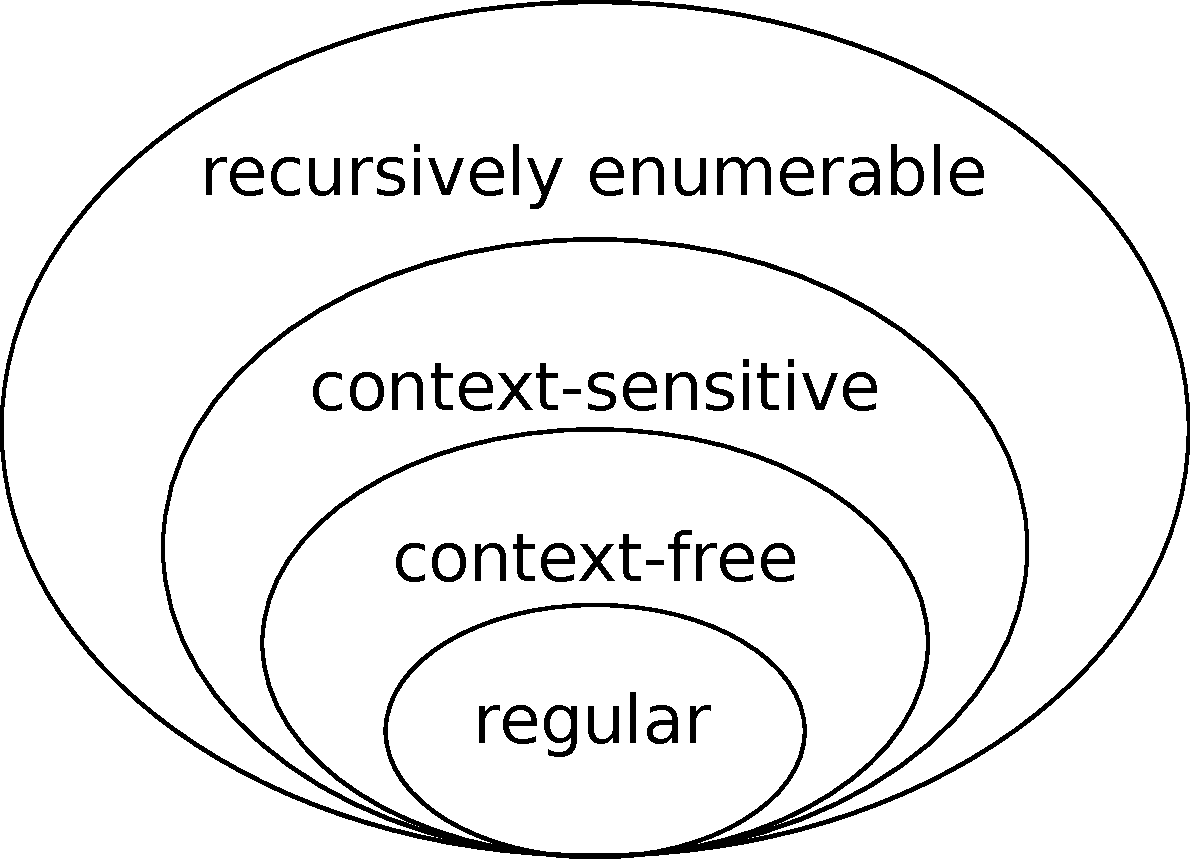
\includegraphics[width=4cm]{Chomsky-hierarchy.pdf}};
\end{tikzpicture}
\end{frame}

\subsection{}
\begin{frame}{Lambda kalkulus}
\begin{itemize}
\item Co program počítá je funkce, která volá jiné funkce, ty volají další funkce\dots
\item Obejdeme se bez globálního stavu, stačí nám parametry!
\item $d(x, y) = x \cdot x + y \cdot y \qquad d(x, y) = {\rm sum}({\rm mul}(x, x), {\rm mul}(y, y))$
\pause
\item Funkce nemusí být pojmenovaná: $\lambda x y \,.\, {\rm sum} \; {\rm mul} \; x \, x \: {\rm mul} \; y \, y$
\pause
\item Funkce může vracet jinou funkci, kterou ``dynamicky vyrobí''
\item Curryfikace: $\lambda x \,.\, \lambda y \,.\, {\rm sum} \;({\rm mul} \;x \,x)\; ({\rm mul}\; y\, y)$
\item $(\lambda x \,.\, (\lambda y \,.\, {\rm sum}\; ({\rm mul}\; x\, x)\; ({\rm mul}\; y\, y))))\: 5\: 10 =$ \\
      $(\lambda y \,.\, {\rm sum}\; ({\rm mul}\; 5\: 5)\; ({\rm mul}\; y\, y))\; 10 =$ \\
      ${\rm sum}\; ({\rm mul}\; 5\: 5)\; ({\rm mul}\; 10\: 10)) = {\rm sum}\; 25\: 100 = 125$
\end{itemize}
\end{frame}

\subsection{}
\begin{frame}{Lambda kalkulus: Mocnost}
\begin{itemize}
\item Churchovy numerály --- $\lambda f \,.\, \lambda x \,.\, x$, $\lambda f \,.\, \lambda x \,.\, f\, x$, $\lambda f \,.\, \lambda x \,.\, f\, f\, x$
\item Podmínky: Booleovské konstanty true $\lambda xy \,\,.\,\, x$, false $\lambda xy \,.\, y$, iszero $\lambda n \,.\, n\; (\lambda x \,.\, {\rm false}) \; {\rm true}$
\item Cykly: Rekurzí --- funkce těla cyklu volá sama sebe, na začátku má podmínku
\pause
\item $f(x) = {\rm iszero}(x, 1, {\rm mul}(x, f(x - 1)))$
\item Ale co když $f$ není pojmenovaná? Předám si ji samu sebe parametrem!
\item $f(x) = f'(f', x) \qquad f'(r, x) = {\rm iszero}(x, 1, {\rm mul}(x, r(x - 1)))$
\item $f\colon g\, g \qquad g\colon \lambda r \,.\, \lambda x \,.\, ({\rm iszero}\; x)\; (1)\; ({\rm mul}\; x\; (r\, ({\rm dec}\; x)))$
\end{itemize}
\end{frame}

\subsection{}
\begin{frame}{Rekurzivní funkce}
\begin{itemize}
\item V $\lambda$-kalkulu jsme oproti ``klasickým matematickým funkcím'' měli syntaktické operátory $\lambda.$
\item To je pohodlné a dá se v něm díky tomu i reálně programovat, ale těžší analýza rekurze
\item Alternativní systém s klasickou matematickou syntaxí
\pause
\item Funkce: $o(x) = 0 \forall x$, $s(x) = x+1 \forall x$, $I^j_n(x_1,\ldots,x_n) = x_j$
\item Operátor substituce: $S_n^m(f,g_1,\ldots,g_m)=h$, $h(x_1,\ldots,x_n) \simeq f(g_1(x_1,\ldots,x_n),\ldots,g_m(x_1,\ldots,x_n))$
\item Operátor prim. rekurze: $R_n(f,g)=h$, $h(0,x_2\ldots,x_n) \simeq f(x_2,\ldots,x_n)$,
	$h(i+1,x_1,\ldots,x_n) \simeq g(i, h(i,x_2,\ldots,x_n), x_2,\ldots,x_n)$
\pause
\item Operátor minimalizace: $M_n(f) = h$, $h(x_1,\ldots,x_n) = z \Leftrightarrow f(x_1,\ldots,x_n,z)=0$ a $z$ je nejmenší
\end{itemize}
\end{frame}

\subsection{}
\begin{frame}{Otázky?}
\begin{center}
{\bf Church-Turingova teze:} Předchozí výpočetní modely \\ (až na konečný automat) jsou {\em univerzální} --- pokrývají \\ všechny ``možné programy'' \\
Ale je {\em vesmír} skutečně takhle výpočetně silný? \\
Dovedete si představit silnější model vy?

\vskip 4ex

Příště: Co {\em nedokážeme} naprogramovat. \\ Podrobněji o rekurzivních funkcích.
\end{center}
\end{frame}

\section{Složitost}
% (Složitost) Úvod do tříd složitosti; P, NP, PSPACE, polynomiální hierarchie.

\subsection{}
\begin{frame}{Algoritmická složitost}
\begin{itemize}
\item Chceme vědět, jak ``rychle'' běží algoritmus --- délka běhu v závislosti na velikosti vstupu
\item Délka běhu je {\em funkce} délky vstupu $f(n)$, která ``asymptoticky odpovídá'' nějaké pěkné funkci $g(n)$
\item $f(n) \in O(g(n)) \Leftrightarrow \exists k > 0, n_0 \forall n_0 \quad |f(n)| \le |g(n) \cdot k|$
\item $O(\cdots)$ je omezení shora, $\Theta(\cdots)$ je omezení shora i sdola
\item Např. $O(1)$, $O(\log n)$, $O(n)$, $O(n\log n)$, $O(n^2)$, $O(2^n)$
\pause
\item Třídy složitosti: Skupina algoritmů se stejnou řádovou složitostí (P, NP, LSPACE, PSPACE, EXPTIME, \dots)
\end{itemize}
\end{frame}

\subsection{}
\begin{frame}{Nedeterministický Turingův stroj}
\begin{itemize}
\item Turingův stroj, který má ``štěstí'' --- z jednoho stavu nepřechází do daného dalšího stavu, ale do množiny stavů
\item Který z množiny? Jeden pohled --- máme orákulum, které vybere stav vedoucí nejkratší cestou do cíle
\item Druhý pohled --- existuje posloupnost voleb stavů, která vede do cíle a splňuje podmínky (třeba polynomiální čas)
\pause
\vskip 3ex
\item Třetí pohled --- ``certifikát'', neboli předložené řešení úlohy, můžeme ověřit v polynomiálním čase
\end{itemize}
\end{frame}

\subsection{}
\begin{frame}{Třídy složitosti}
\begin{itemize}
\item P: Všechny algoritmy, které běží v {\em polynomiálním čase} na deterministickém (``obyčejném'') Turingově stroji
\item NP: Algoritmy, které běží v polynomiálním čase na nedeterministickém Turingově stroji
\item Rovnají se? Co myslíte vy?
\end{itemize}
\end{frame}

\subsection{}
\begin{frame}{Otázky?}
\begin{center}
Příště: Úplné problémy.
\end{center}
\end{frame}

\subsection{}
\begin{frame}{Děkuji vám}
\begin{center}
{\bf pasky@ucw.cz}

Příště: Adaptivní agenti, evoluční algoritmy, \\ datové struktury (haldy), složitost (úplné problémy)
\end{center}
\end{frame}

\end{document}
